%!TEX root = ../template.tex
%%%%%%%%%%%%%%%%%%%%%%%%%%%%%%%%%%%%%%%%%%%%%%%%%%%%%%%%%%%%%%%%%%%%
%% appendix1.tex
%% NOVA thesis document file
%%
%% Chapter with example of appendix with a short dummy text
%%%%%%%%%%%%%%%%%%%%%%%%%%%%%%%%%%%%%%%%%%%%%%%%%%%%%%%%%%%%%%%%%%%%

\typeout{NT FILE appendix1.tex}%

\chapter{Appendix}
\label{app:intro}



\section{Comment Configuration}
\label{app:comment}


\subsection{Comment Configuration Example 1}

\begin{figure}[htbp]
	\centering
	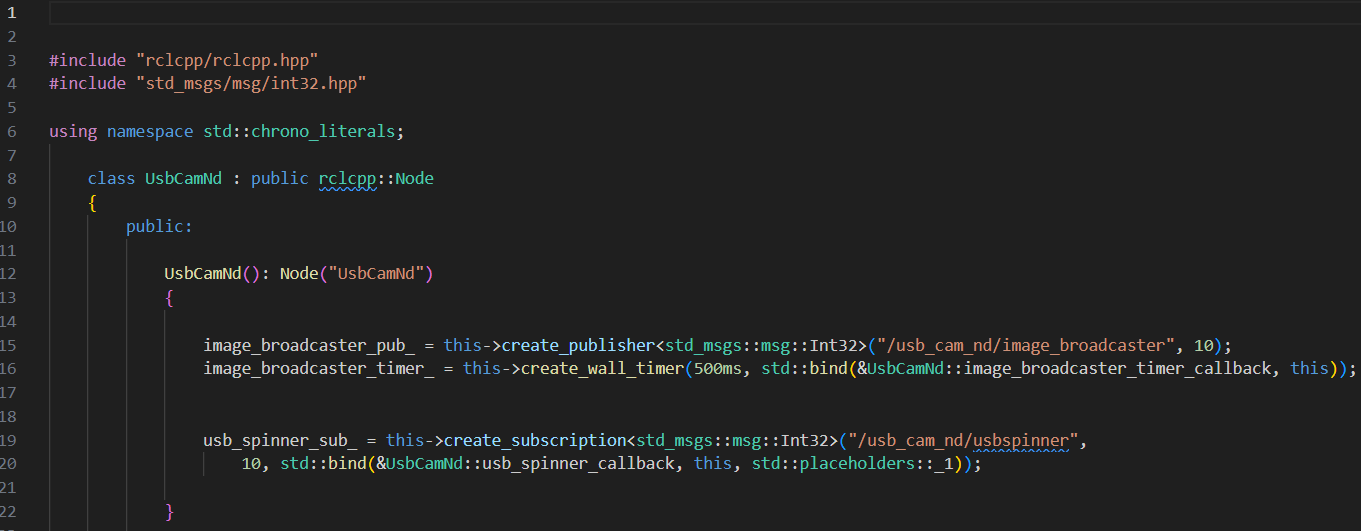
\includegraphics[width=\textwidth]{nocomment_example1.png}
	\caption{Example of generated code without comments}
	\label{figapp:nocomment_example1}
\end{figure}

When code comments are toggled on, the code from Figure~\ref{figapp:nocomment_example1} becomes the code from Figure~\ref{figapp:comment_example1}

\begin{figure}[htbp]
	\centering
	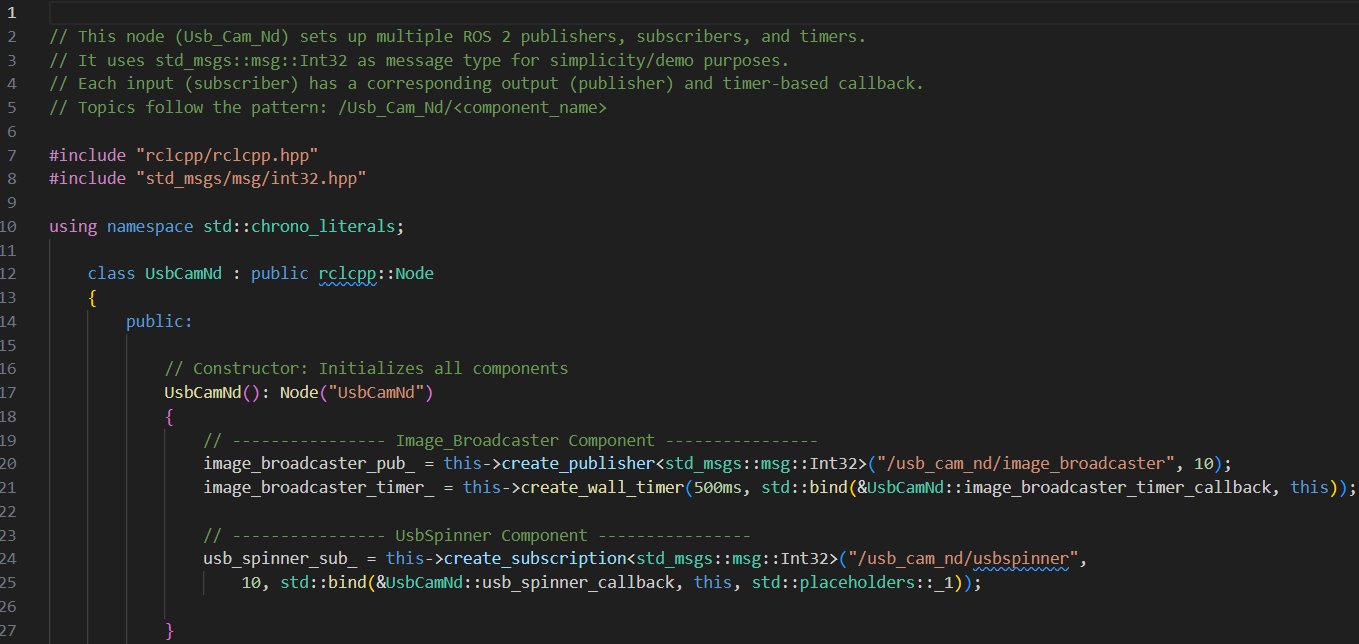
\includegraphics[width=\textwidth]{comment_example1.png}
	\caption{Example of generated code with comments}
	\label{figapp:comment_example1}
\end{figure}


\newpage

\section{Integration and Regression Tests}
\label{app:int_and_reg_tests}


\bgroup
\rowcolors{1}{}{GhostWhite}
\begin{xltabular}{\textwidth}{X X X}
	\caption{Feature dependency table}
	\label{tab:app_int_and_reg_tests}\\
	\toprule
	\rowcolor{Gainsboro}%
	Feature & Depends On & Notes \\
	\midrule
	\Glspl{identifier} & – & Core to code structure \\
	Comments & \Glspl{identifier} & Cheap to implement early \\
	Traceability & \Glspl{identifier}, Comments & Hard to retrofit later \\
	Report & Traceability & Uses trace data \\
	Standard\par Compliance & Report, Traceability & Enforce compliance early \\
	Dead Code\par Elimination & Traceability, Report & Needs stable generation logic \\
	Memory\par Optimization & Dead Code Elim, Traceability & Impacts data structures directly \\
	Node Interface & Memory Optimization & Enables \gls{ROS} decoupling \\
	Legacy Code\par Integration & Node Interface & Most architecture-dependent \\
	\bottomrule
\end{xltabular}


\section{Workflow Execution Time Runs}
\label{app:workflow_exec_time}


\bgroup
\rowcolors{1}{}{GhostWhite}
\begin{xltabular}{\textwidth}{X X X X X X X X X X}
	\caption{First run of workflow execution times (in ms) for an average model with the set of configs from~\ref{app:config_first_batch}}
	\label{tab:workflow_exec_times_1}\\
	\toprule
	\rowcolor{Gainsboro}%
Run & Code & Launch & CMake & Package & Trace & Report & Total Steps & Total & Project Time \\
\midrule
1  & 194 & 65 & 54 & 35 & 92 & 208 & 648 & 663 & 348 \\
2  & 183 & 88 & 58 & 30 & 85 & 205 & 649 & 674 & 359 \\
3  & 138 & 64 & 49 & 34 & 81 & 185 & 551 & 568 & 285 \\
4  & 119 & 50 & 38 & 26 & 74 & 159 & 466 & 477 & 233 \\
5  & 113 & 51 & 43 & 36 & 76 & 163 & 482 & 495 & 243 \\
6  & 104 & 67 & 38 & 27 & 66 & 178 & 480 & 491 & 236 \\
7  & 103 & 43 & 34 & 24 & 66 & 147 & 417 & 425 & 204 \\
8  & 96  & 45 & 38 & 26 & 77 & 142 & 424 & 438 & 205 \\
9  & 89  & 40 & 34 & 24 & 71 & 145 & 403 & 414 & 187 \\
10 & 89  & 45 & 35 & 24 & 70 & 154 & 417 & 426 & 193 \\
11 & 93  & 42 & 34 & 22 & 65 & 162 & 418 & 425 & 191 \\
12 & 86  & 60 & 35 & 25 & 68 & 151 & 425 & 437 & 206 \\
13 & 94  & 52 & 37 & 27 & 67 & 153 & 430 & 438 & 210 \\
14 & 89  & 41 & 34 & 23 & 62 & 155 & 404 & 413 & 187 \\
15 & 87  & 42 & 34 & 24 & 65 & 153 & 405 & 415 & 187 \\
\bottomrule
\end{xltabular}



\section{Generator Configuration Options}
\label{app:configs}


\subsection*{Complete Project Configuration}
\label{app:config_first_batch}

\begin{description}
	\item[Naming]
	\begin{description}
		\item[Style:] \texttt{STANDARD}
		\item[Affix:] \texttt{Telecom\_}
		\item[Affix position:] \texttt{PREFIX}
	\end{description}
	
	\item[Report]
	\begin{description}
		\item[Generate:] \texttt{true}
		\item[Include traceability:] \texttt{true}
		\item[Include summary tables:] \texttt{true}
		\item[Include ROS summaries:] \texttt{true}
		\item[Show detected errors:] \texttt{true}
	\end{description}
	
	\item[Decoupling] Enabled
	
	\item[Comments] \texttt{true}
	
	\item[Traceability] \texttt{true}
\end{description}


\subsection{Configuration UML}

\begin{figure}[htbp]
	\centering
	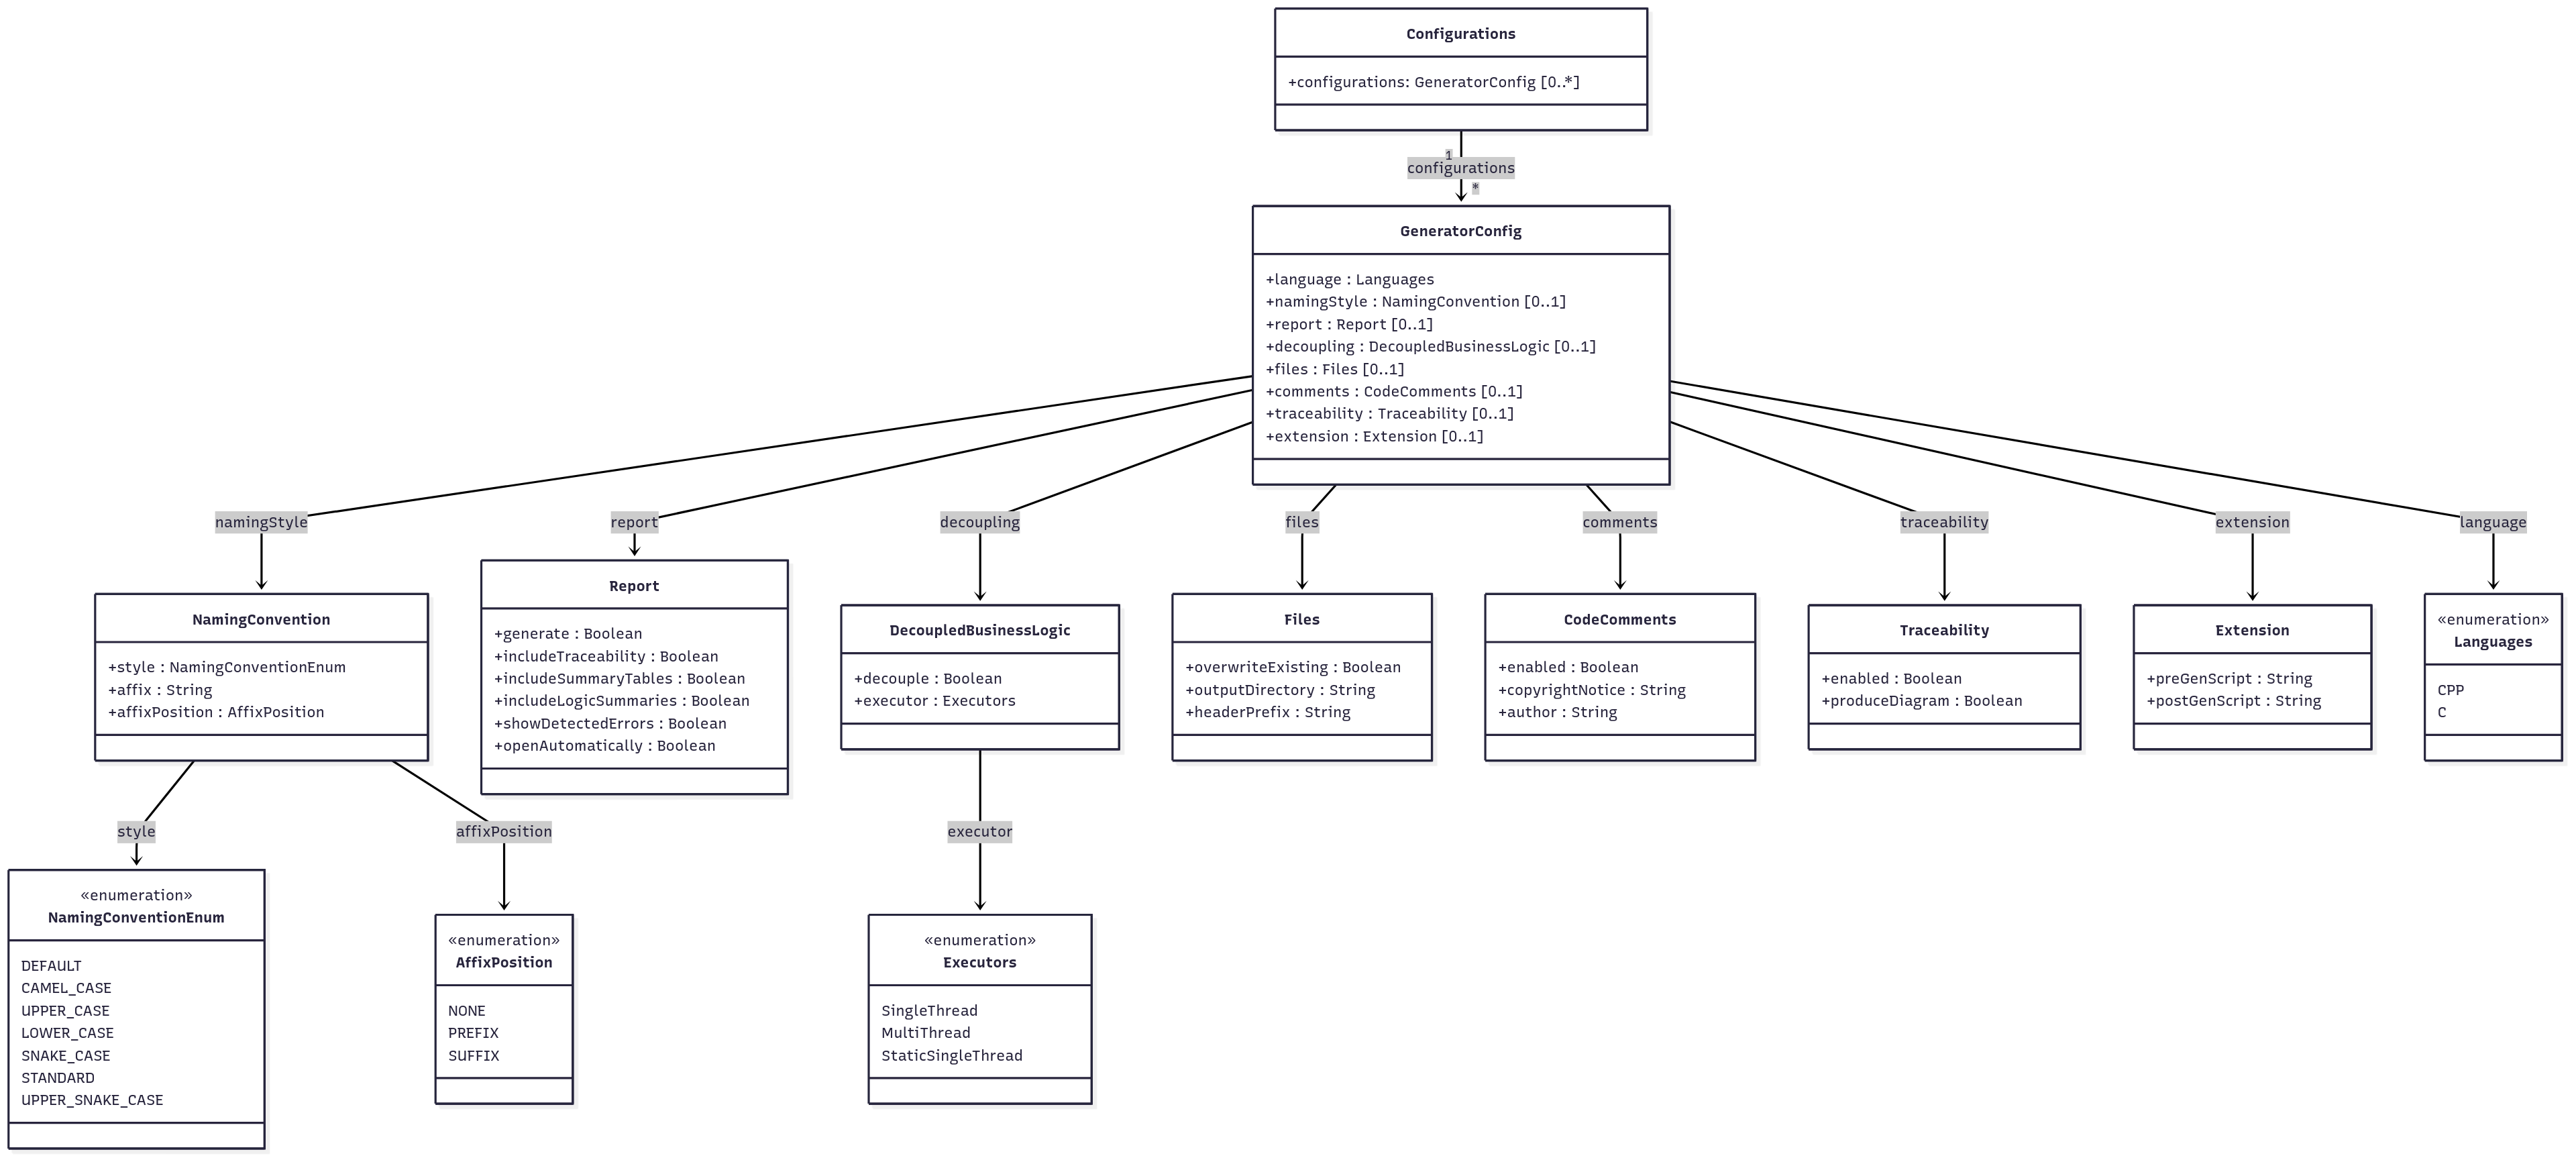
\includegraphics[width=\textwidth]{configLanguageUML.png}
	\caption{UML Diagram of the configuration language, made by the author}
	\label{figapp:configLanguageUML}
\end{figure}

\begin{figure}[htbp]
\centering
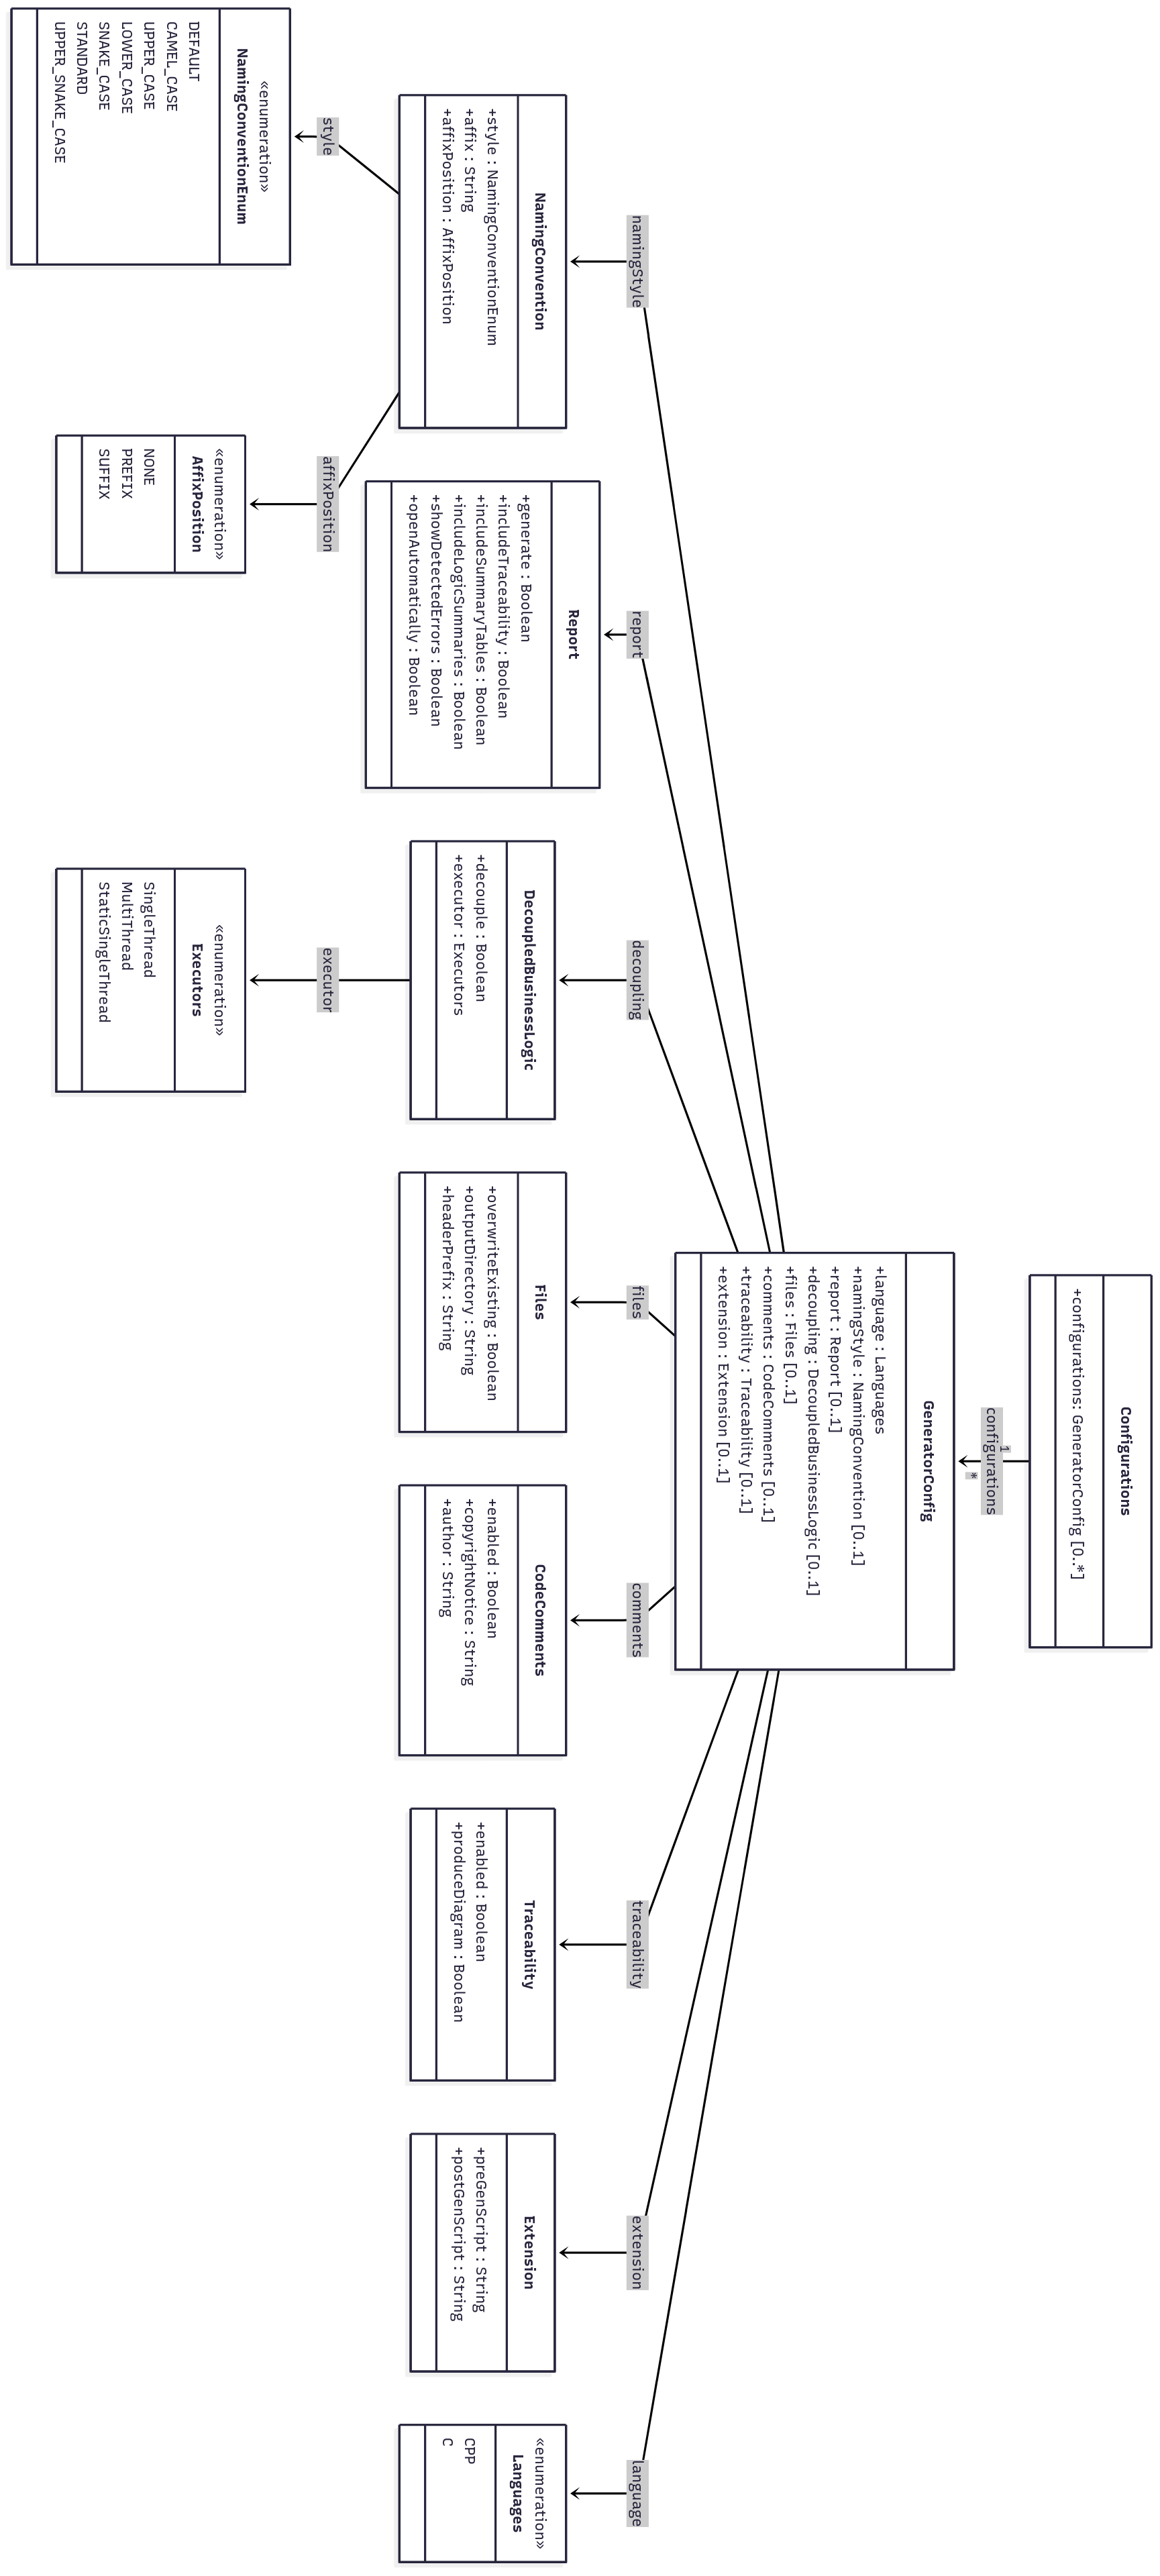
\includegraphics[width=0.7\textwidth]{configLanguageUMLRotated.png}
\caption{UML Diagram of the configuration language rotated 90 degrees for better view}
\label{figapp:configLanguageUMLRotated}
\end{figure}


\newpage

\section{Tests}
\label{app:unit_tests}


\bgroup
\rowcolors{1}{}{GhostWhite}
\begin{xltabular}{\textwidth}{X X X}
	\caption{Code generation verification tests}
	\label{tab:codegen_tests}\\
	\toprule
	\rowcolor{Gainsboro}%
	Test Case ID & Feature & Description \\
	\midrule
	TC-CG-01 & ROS Package Structure & Verify presence of expected folders (\texttt{src}, \texttt{src/launch}) and required files (\texttt{CMakeLists.txt}, \texttt{package.xml}, \texttt{launch.xml}). \\
	TC-CG-02 & Source Code Equivalence & Compare generated \texttt{src} folder with control reference. \\
	TC-CG-03 & Launch File Equivalence & Compare generated \texttt{launch.xml} with control reference at node/remap level. \\
	TC-CG-04 & CMake Consistency & Compare generated \texttt{CMakeLists.txt} with expected reference. \\
	TC-CG-05 & Package Metadata & Compare generated \texttt{package.xml} with expected reference. \\
	TC-CG-06 & Trace Output & Verify \texttt{trace.json} against control reference. \\
	TC-CG-07 & HTML Report & Compare generated report (\texttt{report.html}) with expected. \\
	TC-CG-08 & Static Analysis Report & Compare generated \texttt{cppcheck-report.xml} with control reference. \\
	TC-CG-09 & Node–CMake Consistency & Ensure executables referenced in \texttt{launch.xml} are defined as targets in \texttt{CMakeLists.txt} (with optional \_Node suffix).  \\
	TC-CG-10 & Colcon Build (Disabled) & Attempt build of generated workspace using \texttt{colcon}. Currently disabled due to environment constraints. \\
	\bottomrule
\end{xltabular}
\egroup


\subsection{Unit test execution times}
\label{app:unit_test_times}

\begingroup
\rowcolors{1}{}{GhostWhite}
\begin{xltabular}{\textwidth}{X X X X}
	\caption{Test execution times for standalone and plugin tests}
	\label{tab:test_times}\\
	\toprule
	\rowcolor{Gainsboro}%
	Test Group & Run & Standalone Time (s) & Plugin Time (s) \\
	\midrule
	1 test & 1 & 7.16 & 16.81 \\
	& 2 & 5.58 & 17.90 \\
	& 3 & 5.42 & 18.06 \\
	& 4 & 5.55 & 16.30 \\
	& 5 & 5.42 & 16.32 \\
	\midrule
	10 tests & 1 & 18.59 & 28.07 \\
	\midrule
	20 tests & 1 & 27.84 & 35.97 \\
	& 2 & 28.01 & 36.31 \\
	\midrule
	50 tests & 1 & 34.29 & 41.45 \\
	& 2 & 34.27 & 41.76 \\
	\midrule
	>100 tests & 1 & 63.69 & 71.45 \\
	& 2 & 64.91 & 73.62 \\
	& 3 & 64.87 & 72.26 \\
	\bottomrule
\end{xltabular}
\endgroup







